\chapter{Introduction}
\label{chap:intro}

\section{Kinetic transport equations}

The purpose of this dissertation is to investigate the viability of certain bases for the numerical solution
of {\em kinetic transport equations}. These equations describe transport of energy (by electromagnetic
radiation, say) or particles by means of a density function $u$ which is defined on the phase space,
\[
    u \defeq u(t,\Bx,\Bv)
\]
where $\Bx\in\Omega\subset\bbR^d$ is a spatial coordinate vector, $\Bv\in\cM\subseteq\bbR^d$ denotes velocity
and $t\in[0,\infty)$ is time. We will assume that the spatial domain $\Omega$ is bounded, with nonzero
$d$-dimensional measure, and that the set $\cM\subseteq\bbR^d$ of allowable velocities is a manifold in
$\bbR^d$ of dimension $\dim(\cM) = d_\cM \leq d$.

One may then interpret $u(t,\Bx,\Bv)$ as the $d+d_\cM$-dimensional density of particles located at point $\Bx$
at time $t$ with velocity $\Bv$, or $u(t,\Bx,\Bv)\cdot\Bv$ as the energy flux at point $\Bx$ in direction
$\Bv$ at time $t$.

The general form of kinetic transport equation is
\begin{equation} \label{eqn:kintr}
    \frac{\partial u}{\partial t} + \Bv \cdot \nabla_\Bx u + \kappa u = S(u) + f.
\end{equation}
This equation models the following physical effects:
\begin{itemize}
\item Transport, as realized by the term $\Bv\cdot\nabla_\Bx u$, which moves particles with velocity $\Bv$ in
the direction of $\Bx\to\Bx+\Bv\Delta t$.
\item Absorption or reaction, indicated by the absorption coefficient $\kappa(t,\Bx,\Bv) \geq 0$, which
represents the removal of energy or particles from the system at a rate proportional to the density.
\item Source effects, as denoted by $f(t,\Bx,\Bv)$, which represents the removal (if $f < 0$) or introduction
(if $f > 0$) of energy or particles at a fixed rate independent of the density, but which may depend on time,
space and velocity.
\item Scattering effects, given by the scattering operator $S$, which is often assumed to be linear if $\cM$
is compact,
\begin{equation} \label{eqn:linscat}
    S(u) = \frac{\sigma}{\mu_{d_\cM}(\cM)}\int_\cM \Phi(\Bv,\Bv') u(\Bv') \dd\Bv' - \sigma u,
\end{equation}
where $\mu_d$ is the $d$-dimensional Lebesgue measure. Here $\Phi(\Bv,\Bv')$ is the {\em scattering kernel},
which yields the frequency at which particles with velocity $\Bv'$ obtain a new velocity $\Bv$, and which
is normalized through
\[
    \int_\cM \Phi(\Bv,\Bv') \dd\Bv = 1
\]
for all $\Bv'$. The two terms in \eqref{eqn:linscat} represent {\em gain} and {\em loss} of particles moving
in direction $\Bv$ respectively. In our work we will instead employ nonlinear Boltzmann scattering, to will
be introduced shortly.
\end{itemize}

Assuming fully absorbing walls, we also require the particle density to be prescribed for all incoming
directions at the boundary $\partial\Omega$. That is,
\[
    u(t,\Bx,\Bv) = u_0(t,\Bx,\Bv), \qquad (\Bx,\Bv) \in \Gamma_- \defeq
    \{ (\Bx,\Bv) \in \partial\Omega \times \cM \;:\; \Bv \cdot \Bn(\Bx) \leq 0 \},
\]
where $\Bn(\Bx)$ is the outward facing normal vector at any point $\Bx \in \partial\Omega$. It is also possible
to impose periodic boundary conditions, and we will do so in Chapter~\ref{chap:shearlets}.

\section{The Boltzmann collision operator} \label{sec:boltzmann-intro}

The nonlinear Boltzmann collision operator is defined for distributions on the non-compact velocity space
$\cM=\bbR^d$ as $S(u)=Q(u,u)$, where $Q$ is the bilinear operator
\begin{equation} \label{eqn:Q-std}
  Q(f,h)(\Bv) = \int_{\bbR^d}\int_{\bbS^{d-1}}
  B(|\Bv-\Bv_*|,\cos\theta)(h_*'f'-h_*f)\dd\Bsig \dd \Bv_*, 
\end{equation}
and where the notation $Q(f,h)(\Bv)$ means $Q(f,h)$ evaluated at $\Bv$. We have used the common shorthand
notation 
\[
    f=f(\Bv),\qquad h_*=h(\Bv_*),\qquad f'=f(\Bv'),\qquad h_*' = h(\Bv_*'). 
\]
Since $Q$ acts pointwise in space and time, these variables can be considered as parameters, and they have
been dropped for the sake of readability. The pre- and post-collisional velocities $(\Bv,\Bv_{*})$ and
$(\Bv',\Bv_{*}')$ are related through conservation of momentum and energy,
\[
    \Bv+\Bv_\ast = \Bv'+\Bv_\ast', \qquad |\Bv|^2 + |\Bv_\ast|^2 = |\Bv'|^2 + |\Bv_\ast'|^2.
\]
The solutions to these $d+1$ equations can be parametrized by a unit vector $\Bsigma \in \bbS^{d-1}$ as
\[ 
    \Bv' = \frac{1}{2}\left(\Bv+\Bv_*+|\Bv-\Bv_*|\Bsig\right),\qquad
    \Bv_*' = \frac{1}{2}\left(\Bv+\Bv_*-|\Bv-\Bv_*|\Bsig\right).
\]
See Figure~\ref{fig:boltzmann-sphere}.

\begin{figure}
    \centering
    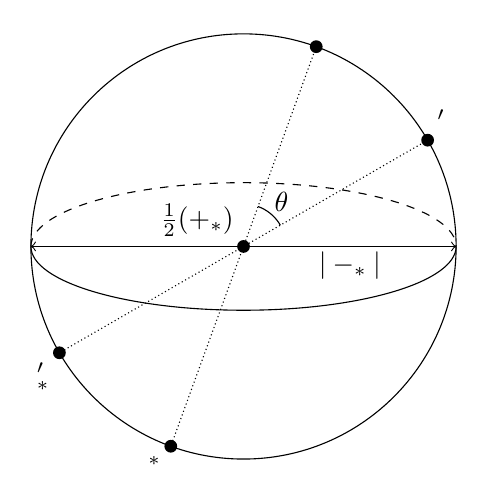
\begin{tikzpicture}[scale=2.7]
        \coordinate[label=70:$\Bv$] (pr) at (70:1);
        \coordinate[label=250:$\Bv_\ast$] (prs) at (250:1);
        \coordinate[label=30:$\Bv'$] (po) at (30:1);
        \coordinate[label=210:$\Bv_\ast'$] (pos) at (210:1);
        \coordinate[label={[label distance=-0.12cm]50:$\theta$}] (bs) at (50:0.2);
        \coordinate[label=135:$\frac{1}{2}(\Bv+\Bv_\ast)$] (center) at (0,0);
        \coordinate[label={[label distance=-0.06cm]270:$|\Bv-\Bv_\ast|$}] (midrad) at (0:0.5);

        \draw (-1,0) arc (180:360:1cm and 0.3cm);
        \draw[dashed] (-1,0) arc (180:0:1cm and 0.3cm);
        \draw (0,0) circle (1cm);

        \draw[densely dotted] (pr) -- (prs);
        \draw[densely dotted] (po) -- (pos);

        \draw (30:0.2) arc (30:70:0.2);
        \draw[<->] (180:1) -- (0:1);

        \fill (pr) circle (0.03);
        \fill (prs) circle (0.03);
        \fill (po) circle (0.03);
        \fill (pos) circle (0.03);
        \fill (center) circle (0.03);
    \end{tikzpicture}
    \caption{Illustrating the relationship between pre- and post-collisional velocities. On a sphere centered
        at $\nicefrac{1}{2}\left(\Bv+\Bv_\ast\right)$ with diameter $|\Bv-\Bv_\ast|$, the pre-collisional
        velocities are diametrically opposite, as are the post-collisional velocities. The angle between the
        two is the $\theta$ entering \eqref{eqn:Q-std}.}
    \label{fig:boltzmann-sphere}
\end{figure}

For the Boltzmann operator, the two terms $h_*'f'$ and $h_*f$ are called {\em gain} and {\em loss} parts
respectively, and it is often useful (and we will do so when necessary) to split the collision operator and
write
\[
    Q(f,h) = Q^{+}(f,h) - Q^{-}(f,h). 
\]
For the physical background and mathematical analysis of this
operator, we refer to
\cite{Cercignani2002bef,Villani2002rmt}. Throughout this paper we make
the following customary assumption on the collision kernel $B$ in
\eqref{eqn:Q-std}.
\begin{assumption} \label{ass:B} Assume that $B$ is separable, with a power law dependence on the relative
    velocity, that is,
\begin{equation}\label{eq:CrossRep}
    B(|\Bu|,\cos\theta) = |\Bu|^\lambda b(\cos\theta),\qquad
        \text{with}\quad \lambda\geq-\frac{d}{2},
\end{equation}
and some function $b:[-1,1]\to\mathbb{R}$ that satisfies {\em Grad's cutoff assumption}
\begin{equation}\label{eq:Grad}
  \int_{\bbS^{d-1}}b(\cos\theta) \dd\Bsigma < \infty.
\end{equation}
\end{assumption}
The assumption on the form of $B$ is not restrictive. It includes, for example, all kernels arising from
inverse power law forces between particles, as well as the hard spheres kernel (with $\lambda=1,b\equiv0$).

The most significant feature about the function $b$ is a non-integrable singularity at $\cos\theta=1$, which
has been cut off in \eqref{eq:Grad}. This assumption greatly simplifies the analysis of the mathematical
properties of $Q$.

The collision operator \eqref{eqn:Q-std} conserves the following important quantities:
\begin{align*}
    \text{Mass density:} &\qquad\rho(g) = \int_{\bbR^d} g(\Bv)\dd\Bv,\\
    \text{Momentum:} &\qquad \Bu(g) = \frac{1}{\rho(g)}\int_{\bbR^d} g(\Bv)\Bv\dd\Bv,\\
    \text{Energy:} &\qquad E(g) = \frac{1}{\rho(g)}\int_{\bbR^d} g(\Bv)|\Bv|^2\dd\Bv,\\
    \text{Temperature:} &\qquad T(g) = \frac{1}{d\rho(g)}\int_{\bbR^d} g(\Bu(g)+\Bv)|\Bv|^2\dd\Bv.
\end{align*}
One observes the following relationship between energy, temperature and momentum:
\[
    E(g) = dT(g) + |\Bu(g)|^2.
\]
In fact, $T$ is invariant with respect to translations, a convenient enough property that one often prefers to
work with temperature instead of energy.

Solutions to the {\em spatially homogeneous} Boltzmann equation 
\[
    \frac{\partial f}{\partial t} = Q(f,f)
\]
converge to Maxwellian distributions (see for example
\cite{Gressman2011gcs} for recent work on this property), which are
fully determined by the observables $\rho$, $\Bu$ and $T$ (or $E$):
\begin{equation} \label{eqn:maxwellian}
    \mu(\Bv) = \frac{\rho}{(2\pi T)^{\nicefrac{d}{2}}} \exp\left( -\frac{|\Bv-\Bu|^2}{2T} \right).
\end{equation}
The following properties of $Q$ are particularly important.
\begin{theorem} \label{thm:trans-rot-Q}
For $\Bc\in\bbR^d$, let $\tau_\Bc$ be a translation operator, i.e. $\tau_\Bc f(\Bx) = f(\Bx-\Bc)$. Also, given a
rotation matrix $R\in\bbR^{d\times d}$, let $\rho_R$ be a rotation operator, i.e. $\rho_R f(\Bx) = f(R\Bx)$.
Then $Q$ commutes with $\tau_\Bc$ and $\rho_R$:
\[
    Q(\tau_\Bc f, \tau_\Bc g) = \tau_\Bc Q(f,g), \qquad
    Q(\rho_R f, \rho_R g) = \rho_R Q(f,g).
\]
\end{theorem}
Theorem \ref{thm:trans-rot-Q} is important to the viability of both the Fourier discretization developed in
Chapter~\ref{chap:boltzmann-fourier} and the polar Laguerre method developed in
Chapter~\ref{chap:boltzmann-polar}.

\section{Variations on kinetic transport}

Different varieties of \eqref{eqn:kintr} arise through variation of the parameters $\kappa$, $\Phi$,
$\sigma$ and $f$, the scattering operator $S$, and the domains $\Omega$ and $\cM$. Some other variations to
consider are
\begin{itemize}
\item {\bf Stationary solutions}, which assume $\partial_t u = 0$, and so we obtain
\[
    \Bv\cdot\nabla_\Bx u + \kappa u = S(u) + f
\]
with no change in boundary conditions.
\item {\bf Pre-imposed velocity fields}. This is a special case of the more general formulation where the
velocity manifold $\cM$ may depend on $\Bx$. Specifically, it is assumed to be a singleton $\cM(\Bx) = \{
\Bv(\Bx) \}$, and so all particles at point $\Bx$ have the same velocity $\Bv$. The equation then reads
\[
    \frac{\partial u}{\partial t} + \Bv(\Bx)\cdot\nabla_\Bx u + \kappa u = f
\]
where $u \defeq u(t,\Bx)$ (this is the equation for single-speed neutron transport, or monochromatic radiative
transfer). Scattering makes no sense here, so it has been removed. Boundary conditions still need to be
imposed on the inflow boundary, which takes the form
\[
    \Gamma_- = \{ \Bx \in \partial\Omega \;:\: \Bv(\Bx) \cdot \Bn(\Bx) \leq 0 \}.
\]
\item {\bf Spatial homogeneity}. In this formulation, $u$ is assumed to have identical velocity distributions
at all points $\Bx\in\Omega$. In particular, the transport term will disappear, giving
\[
    \frac{\partial u}{\partial t} + \kappa u = S(u) + f
\]
where $u \defeq u(t,\Bv)$. In this case, no boundary conditions are needed to achieve
uniqueness.\footnote{Except, of course, initial conditions for $t=0$.}
\end{itemize}

In the case of linear scattering and a velocity manifold with uniform speeds (where $\cM$ is the unit sphere
$\bbS^{d-1}$), we obtain the neutron transport equation, also known as the monochromatic radiative transfer
equation.\footnote{One can extend the formulation to also let $u$ depend on $\nu\in\cF$, where $\cF$ is a set
of allowable frequencies. The scattering operator may be modified to allow particles to also change
frequency.}

In this dissertation, we will consider two other variations of \eqref{eqn:kintr}, with very different
characteristics. In Chapter~\ref{chap:shearlets} we will study the stationary advection-reaction equation,
\[
    \Bv(\Bx)\cdot\nabla_\Bx u + \kappa u = f,
\]
with periodic or inflow boundary conditions, and in Chapters \ref{chap:boltzmann-fourier} and
\ref{chap:boltzmann-polar} we will study the spatially homogeneous Boltzmann equation
\[
    \frac{\partial f}{\partial t} = Q(f,f),
\]
with no boundary conditions and $\cM=\bbR^d$, where $Q$ is the nonlinear Boltzmann collision operator which
has been introduced in Section~\ref{sec:boltzmann-intro}. It is customary to use $f$ as the unknown function
in Boltzmann circles, and so we will follow this convention.

\section{Discretization}

In the most general setting, one is faced with the solution of a $1+d+d_\cM$-dimensional equation, and in
particular the problem of discretizing a transport and scattering operator in $d+d_\cM$ dimensions. This
quantity can take on values in the interval $[d,2d]$. In particular, if the velocity field is prescribed we
obtain a $d$-dimensional problem, for the radiative transfer equation we have a $2d-1$-dimensional problem,
and for the Boltzmann equation we have the full $2d$ dimensions.

Of obvious interest are three-dimensional simulations, which means we must be prepared to solve equations in
six dimensions. Due to the now (in)famous ``curse of dimensionality'', this is a nontrivial issue.  Under a
traditional finite element discretization with $N$ degrees of freedom in each direction (i.e. a total of
$\cO(N^{d_\rms})$ for a $d_\rms$-dimensional problem), we obtain an asymptotic error rate of
$\cO(N^{-\nicefrac{p}{d_\rms}})$ if the solution is of smoothness order $p$ and the finite element spaces are
of sufficiently high order to capture this.

In general, solutions to kinetic transport equations do not display particularly high smoothness, and so with
a problem of dimension $d_\rms=6$, the convergence will slow to a crawl in the number of degrees of freedom.

Sparse grids were introduced in the context of finite element methods by \cite{Zenger1991pap} and have proven
useful in solving several PDEs, monochromatic radiative transfer equation among them \cite{Widmer2008saf}. The idea
is that if the $d_\rms$-dimensional problem can be formulated on a product domain $\Omega = \Omega_1 \times
\Omega_2$, where the dimension of $\Omega_i$ is $d_i$, we can achieve the same asymptotic error (up to
logarithmic terms), with a substantial reduction of degrees of freedom, namely
\[
    \cO\left(N^{d_\rmm} \left(\log N\right)^{d_\rmm} \right), \qquad d_\rmm = \max\{d_1,d_2\}.
\]
The prerequisites for this construction are the tensor product domain, a higher smoothness condition on the
solution (involving mixed derivatives), and the formulation of multilevel hierarchical bases on the subdomains.

Our primary objective in this dissertation is the latter point, namely to investigate possible function spaces
on the physical domain $\Omega$ and the velocity manifold $\cM$. It is for this reason that we will study the
stationary advection-reaction equation (which does not have a velocity space), and the spatially homogeneous
Boltzmann equation (which, correspondingly, does not have a physical space). This reduction in complexity will
allow us to focus more easily on the relevant subspaces.

It is worth noting that since the domains $\Omega$ and $\cM$ do not generally admit tensor product structures,
the sparse grids approach halts at this point. In the cases that they do, it is worth considering. This is in
fact the case for the Boltzmann equation, where $\cM=\bbR^d$. We will make use of this fact in formulating the
hyperbolic cross method in Chapter~\ref{chap:boltzmann-fourier}.

\section{Overview of the dissertation}

In Chapter~\ref{chap:shearlets} we perform a limited study of shearlet-based function spaces for use in
discretizing the physical domain of the stationary advection-reaction equation. This discussion is focused
heavily on implementation, since shearlets are a recent innovation and have not been used previously for
solving PDEs.

In Chapter~\ref{chap:boltzmann-fourier} we investigate a hyperbolic cross Fourier spectral discretization for
the spatially homogeneous Boltzmann equation, which may be considered a sparse version of the {\em de facto}
standard method for this problem (the full-grid Fourier spectral discretization). We provide an in-depth
analysis of this method, and provide analogues for several results that have already been established for the
more standard Fourier methods.

In Chapter~\ref{chap:boltzmann-polar} we develop for the spatially homogeneous Boltzmann equation a novel
polar function space based on Laguerre polynomials, which has prior to this only been used for fully
rotationally symmetric solutions.

Aside from the theoretical analysis of the sparse Fourier method in Section~\ref{sec:appr}, this dissertation
is algorithmic in nature. Appendices are provided with code listings for the methods of Chapters
\ref{chap:shearlets} and \ref{chap:boltzmann-polar}. As a consequence of this focus, we rely mostly on
numerical experiments to evaluate the performance of the methods described. Some results are shown which rely
on unproven but probable assumptions (specifically those in Section~\ref{sec:evolerr} relying on
Conjecture~\vref{ass:decay}), and some theoretical work is left for the future, in particular the analysis of
the polar Laguerre method of Chapter~\ref{chap:boltzmann-polar}.

Aside from the present discussion, Chapter~\ref{chap:shearlets} may be considered effectively disjoint from
Chapters \ref{chap:boltzmann-fourier} and \ref{chap:boltzmann-polar}. The latter two chapters overlap only
insofar as they discuss methods for solving the same equation.
